\documentclass[]{aastex62}
\usepackage{amssymb,amsmath}

 
\newcommand{\vk}{von K\'{a}rm\'{a}n}
\newcommand{\vdag}{(v)^\dagger}
\newcommand\aastex{AAS\TeX}
\newcommand\latex{La\TeX}


\def\eq#1{\begin{equation} #1 \end{equation}}
\def\mic              {\hbox{$\mu\mathrm{m}$}}
\def\atm    {\hbox{\rm{ATM}}}

\graphicspath{{./}{figures/}}
 
\shorttitle{Hot and Cold SOC-i Cases}
\shortauthors{Tate \& Ivezi\'{c}}

\begin{document}

\title{Hot and Cold Cases for SOC-i Thermal Analysis (v1)}  
 
%\email{ivezic@uw.edu}

\author{Boone Tate, \v{Z}eljko Ivezi\'{c}}
\affiliation{University of Washington, 3910 15th Avenue NE, Seattle, WA 98195, USA}

\begin{abstract}
We computed temperature variation with time for the SOC-i satellite using a variety of input
assumptions. The computation is based on a simple model for the satellite temperature variation 
with time when the satellite is subjected to a bistable heat source: two orbital segments with 
piece-wise constant power. The model assumes that at a given time a single temperature applies 
to the entire satellite body. 
We defined the so-called ``hot'' and ``cold'' cases and found that the low and high temperature 
extremes for a randomly oriented SOC-i satellite are $-$14 $^\circ$C and $+$17 $^\circ$C. When the 
satellite orientation is deliberately chosen to maximize the temperature extremes, the corresponding 
values are $-$38 $^\circ$C and $+$42 $^\circ$C. These results, and the allowed operating temperature
ranges for satellite components imply that low temperatures will be more worrisome than high
temperatures. We also explored a toy model for active temperature control that assumes an additional
internal power dissipation whenever the satellite temperature drops below a pre-defined threshold,
and concluded that such an approach is a viable method for mitigating low temperatures.
These results are sensitive to assumed specific heat, which we simply assumed to correspond to 
aluminum, and should be revisited with more accurate input values. 
\end{abstract}

\keywords{Satellites --- CubeSat --- SOC-i --- Radiative transfer --- Thermal model}


\section{Introduction}
 
When designing a satellite such as SOC-i, it is crucial to establish that the temperature variation for 
each component will be within its operating range. In practice, professional engineering tools and 
numerical analysis are used to analyze complex systems. The SOC-i team utilizes the code Ansys
to predict satellites temperature distribution. In order to compute temperatures, Ansys requires
as input numerical specifications for the sources of radiation that SOC-i absorbs. In addition, 
the satellite's orbital parameters and orientation are also required. Given that the details of 
SOC-i orbit will not be known until its launch, here we define the so-called ``hot'' and ``cold'' 
cases which capture scenarios that predict the coldest and the hottest satellite temperatures. 
 
In addition, we computed SOC-i temperature variation with time for hot and cold cases using
a simple model that assumes that a single temperature applies to the entire satellite body 
at any given time. Although simple, this modeling produces approximately correct temperature
estimates and deep physical insight, and can be used for fast studies of the impact of various
input assumptions on the resulting satellite temperature. Most importantly, these results 
provide a ``sanity check'' for the more sophisticated, but also more prone to input errors, 
Ansys models.
 
The main quantitative result of the models presented here is that it is much more likely 
for low than for high temperatures to present problems for SOC-i operations phase. 
Motivated by this finding, we also explored a toy model for active temperature control that 
assumes an additional internal power dissipation whenever the satellite temperature
drops below a pre-defined threshold. 

In the next section, we first describe our mathematical model and input parameters, and then 
discuss specific results obtained with input parameters corresponding to SOC-i. In \S\ref{sec:active},
we present a toy model for active temperature control, and summarize our findings in \S\ref{sec:conclusions}. 



\section{Thermal Analysis for SOC-i} 

The mathematical model for thermal analysis is discussed in detail in an accompanying document 
(\v{Z}. Ivezi\'{c}, 2021, unpublished, hereafter I21).  Here we extend analysis from a bistable heat source
discussed there to an arbitrary heating pattern along the orbit, including a temperature-driven
additional internal power dissipation. For this reason, we had to resort to a numerical solution
of the governing differential equation (see eq.~1 in I21, hereafter I21-eq1). A sufficient accuracy of numerical 
solution was verified using analytic solution for a case with piecewise constant bistable heat source (I21-eq17). 

Model input parameters include environmental, orbital and satellite parameters, all of them
subject to appreciable uncertainties. At least in principle, orbital and satellite parameters 
are deterministic and should not have any uncertainties. However, detailed orbital information
is sometimes unknown until the launch, and satellite orientation might be subject to 
operational uncertainties. We first describe SOC-i physical parameters used in computations
here, and then discuss orbital and environmental parameters, including definitions of the 
so-called ``hot'' and ``cold'' cases that attempt to account for various modeling uncertainties. 
After all the input parameters are introduced, we discuss the results of thermal modeling. 
 

\subsection{Input satellite parameters}

We used the SOC-i CAD model developed for structural analysis to extract information about
external satellite surfaces and their material properties. We adopted the following description 
of external SOC-i surfaces: 
\begin{itemize}
\item  Top: 60\% solar panel, 40\% aluminum frame
\item  Bottom: 38\% aluminum frame, 62\% PCB (printed circuit board). 
\item  Sides (2): 64\% solar panels, 19\% aluminum panels (outside), 17\% aluminum frame rails
\item  Sides (2): 57\% solar panels, 26\% aluminum panels (outside), 17\% aluminum frame rails
\end{itemize}

With the values of absorptivity and emissivity listed in Table~\ref{tab:inputsAbsEmiss}, we obtained
their surface-weighted values $\alpha=0.83$ and $\epsilon=0.79$ (54\% of external surface area
is covered by solar panels). In addition, we assumed that the satellite mass is $m=2.6$ kg and 
adopted specific heat corresponding to aluminum ($C=768$  J\,kg$^{-1}$\,K$^{-1}$), yielding a
thermal intertia of $mC = 2.00$ kJ\,K$^{-1}$. This value of thermal intertia needs to be varified with 
detailed modeling (e.g., summing the $mC$ product for all individual structural components
in the SOC-i CAD model). 

\begin{table}[t]
	\centering
	\caption{Surface optical absorptivity and infrared emissivity for SOC-i surface materials. }
	\label{tab:inputsAbsEmiss}
	\begin{tabular}{r|r|r|r|r|r} % 
		\hline
  	              Part        &                Surface          &    $\alpha$  &   $\epsilon$    &   $k$ (W\,m$^{-1}$\,K$^{-1}$)   &  $C$ (J\,kg$^{-1}$\,K$^{-1}$)  \\
	  	\hline
         Solar panels        &       GaAs, with AR coating  &           0.92      &          0.85      &   60.6    &      324   \\  
     Al panels, outside   &     7075 Al, Kapton             &           0.87       &         0.81       &  121.2   &    801   \\ 
          Al frame rails    &       5052 Al, hard anodized &          0.86        &        0.86      &    138.5   &    768    \\  
                Al frame      &       5052 Al, alodine            &          0.08        &        0.15       &   138.5   &    768    \\
                PCBs            &               FR4                        &           0.81       &         0.90        &   18.0  &    1544  \\ 
 		\hline     
	\end{tabular} 
\end{table}
 

\subsection{Assumptions for orbital parameters}

It is already known that SOC-i will have a nearly-polar sun-synchronous 
orbit\footnote{See https://en.wikipedia.org/wiki/Sun-synchronous\_orbit} 
with an altitude of $h=550$ km and orbital inclination of 97.7 degrees. A satellite in sun-synchronous 
orbit passes over any given point of the planet's surface at the same local mean solar time because the 
orbit precesses through one complete revolution each year (that is, the orbit always maintains the same 
relationship with the Sun). 

The eclipse duration for sun-synchronous orbits depends on their right ascension of the 
ascending node (RAAN), which will not be known until the launch date (RAAN is determined
by the exact launch time). The orbital period for sun-synchronous orbit with an altitude of 
$h=550$ km is 96 mins, and the maximum eclipse duration is 36 mins.  When the orbital 
plane is perpendicular to incoming solar radiation, there is no eclipse (the satellite is following 
the terminator line at all times). 


\begin{table}[t]
	\centering
	\caption{The range of input enviromental parameters. }
	\label{tab:inputsEnvParam}
	\begin{tabular}{r|r|r|r|r} % 
		\hline
  	         Quantity & max    &   min   &  mean &  unit            \\
		\hline
              Solar flux   &  1422  &  1322  &  1372 & Wm$^{-2}$  \\
           Earth albedo  &    35    &    25    &     30  &   \%            \\ 
            Earth IR flux &  260    &   220   &    240 & Wm$^{-2}$   \\
 		\hline
	\end{tabular} 
\end{table}


\subsection{The concept of hot and cold cases} 

Due to uncertainties in input parameters, including environmental, orbital and satellite parameters,
engineering pre-launch analysis often focuses on most extreme scenarios that predict the coldest 
and the hottest satellite temperatures. We define ``hot'' and ``cold'' cases by first adopting 
the extreme values of environmental parameters from Table~\ref{tab:inputsEnvParam}. 

In addition, we make an assumption that the orientation of SOC-i's sun-synchronous orbit
results in an eclipse with maximum duration (36 min) for cold case, and no eclipse at all for 
hot case. 

The intensity of solar radiation reflected from Earth varies along the orbit (I21-eq6). For a polar 
orbit passing through subsolar point, $f_{alb}=0.62$ for the non-eclipsed part of the orbit, while 
for a polar orbit aligned with the terminator (with no eclipse), $f_{alb}=0.06$. Therefore, 
we adopt $f_{alb}=0.62$ for hot case and $f_{alb}=0.06$ for cold case (note that reflected solar 
radiation contributes more flux for cold case, when not in eclipse). 
 
With these assumptions, we use equations 3--13 from I21 to compute incoming heating flux.
For cold case, the only heating flux during the eclipsed portion of the orbit is IR flux from Earth. 
The variation of flux between hot and cold cases for three main heat sources is summarized in 
Table~\ref{tab:inputflux}. Note that reflected solar flux is smaller for hot case but this difference
is compensated by the absence of eclipsed orbital portion in hot case. 

Table~\ref{tab:inputflux} lists absorbed flux per unit area, assuming SOC-i's effective 
absorption coefficient ($\alpha$). {\bf The listed value are also appropriate for detailed 
Ansys-based modeling, but need to be corrected for $\alpha$ of each surface material.} 
The actual absorbed power (absorbed energy per unit time) depends on 
the values of $\eta_S$ and $\eta_E$, which in turn depend on orientation. We make additional 
assumptions about satellite orientation, as discussed next. 

\begin{table}[t]
	\centering
	\caption{Absorbed flux ($\alpha=0.83$) for hot and cold cases (in  Wm$^{-2}$). }
	\label{tab:inputflux}
	\begin{tabular}{r|r|r|r} % 
		\hline
  	                    Quantity  & hot case   &   cold  case &   ratio hot/cold    \\
		\hline
              Direct solar flux    &    1181        &     1098         &     1.08       \\
           Reflected solar flux  &     21.0        &     144.2        &     0.15     \\    
                       Earth IR flux  &   174.6       &     147.8        &     1.18      \\
		\hline
	\end{tabular} 
\end{table}



\subsection{Assumptions for satellite orientation}

The satellite orientation determines effective surface areas for the absorption of radiation from 
the Sun and Earth. For convenience, these surface areas are expressed relative to the total surface area, $A_{tot}$
(=0.1 m$^2$ for SOC-i), using $\eta$ factors ($\eta_S$ and $\eta_E$, respectively). For a given 
orbit and satellite orientation, $\eta_S$ and $\eta_E$ can be computed by adding corresponding
values (known as ``view factors'') for six individual sides (see Appendix A in I21).  

We used results discussed in Section 2.4 from I21 to adopt the following values for SOC-i.
When averaged over plausible orientations and orbits, $\eta_S = 0.21$ and $\eta_E = 0.36$, 
with an uncertainty due to actual orbit specifics of the order 10\%. The limits of 
possible ranges are  $\eta_S = 0.10 - 0.30$ and $\eta_E = 0.34 - 0.38$. The limits for 
$\eta_S$ reflect the range of projected area towards plane-parallel rays for 2U CubeSat geometry, 
with the minimum value corresponding to one small side oriented perpendicularly to the incoming 
solar radiation. For $\eta_E$, the variation is much smaller because typically all six sides can 
``see'' Earth's surface\footnote{We note that even for spherical geometry $\eta_S$ and $\eta_E$
are generally different:  $\eta_S=1/4$, while $\eta_E$ decreases from 1/2 to 1/4 as the orbit
altitude varies from zero to infinity.}. 
 
We do not adopt specific satellite orientation for hot and cold cases but instead explore two 
options in each case.  First, we adopt averaged orientations for both hot and cold cases,
with $\eta_S = 0.21$ and $\eta_E = 0.36$ corresponding to 2U CubeSat values. As the second 
assumption, we consider the following extreme cases: $\eta_S = 0.30$ and $\eta_E = 0.34$ for 
hot case, and $\eta_S = 0.10$ and $\eta_E = 0.38$ for cold case.  
 
The second set of values assumes that the satellite orientation is actively controlled.  For hot
case, the maximum possible projected satellite area for plane-parallel rays is always pointing 
towards the Sun ($\eta_S = 0.30$). For cold case and during non-eclipsed portion, the smallest 
satellite side is always pointing towards the Sun ($\eta_S = 0.10$).  The adopted values of 
$\eta_E$ are its extreme values. 



\newpage
\subsection{Assumptions for internal power dissipation}


A fraction of absorbed optical flux (the sum of direct solar flux and reflected solar flux) is often 
used to charge on-board batteries. We assume that 20\% of absorbed flux\footnote{Here, $\eta_{cell}$ 
represents the fraction of all absorbed radiation that was converted to battery charge. For example, if 
the cells occupy 2/3 of all external surfaces, and the cell conversion efficiency is 30\%, then $\eta_{cell}$= 0.2. 
For randomized orientiations, it's only ``effective'' quantities that count in the model considered here; 
however, when a specific satellite orientation is known, one could incorporate information about where 
exactly the solar cell panels are positioned, too.} is converted into chemical
energy ($\eta_{cell}=0.2$). This energy is returned back at a constant rate as internal heat dissipation. 

In hot case, satellite is always exposed to the Sun and there is {\bf no net effect} within the context
of single-temperature model considered here. In reality, and in detailed Ansys models, this
internal heat dissipation can modify the temperature distribution within the satellite (areas closer
to the heater will have elevated temperature). In cold case, the effect of internal heat dissipation
is to {\bf minimize} the amplitude of temperature variation, or equivalently, to raise the minimum
temperature (at the end of eclipsed portion). 
 
These assumptions complete the specification of hot and cold thermal models. We proceed
with a discussion of numerical results. 

\begin{table}[t]
	\centering
	\caption{Absorbed power (in Watt) and equilibrium temperatures for hot and cold SOC-i cases. }
	\label{tab:powertemp}
	\begin{tabular}{r|r|r|r|r} % 
		\hline
  	                    Quantity          & hot, random   &  hot, extreme &   cold, random  & cold, extreme   \\
		\hline
           Absorbed direct solar         &  24.8        &  36.6     &  23.1         &  11.0      \\
           Absorbed Earth albedo       &    0.8        &    0.8   &     5.2           &  4.9      \\    
               Absorbed Earth IR           &    6.3        &    6.6     &     5.3        &  5.0     \\
             Internal dissipation           &    5.1        &   7.5     &     3.5         &  2.0     \\
		\hline 
             Total input in eclipse       &     ---      &   ---   &     8.9       &    7.0  \\
              Total input in sun            &    31.8      &   44.0  &   31.4        &  19.7  \\
		\hline
              Equilibrium T in eclipse  &     ---     &    ---   &    211       &   199 \\
              Equilibrium T in sun       &      290      &   315   &    289        &  257  \\
 		\hline
                    $T_{min}$  (K)               &      290      &   315   &   259       &  235  \\
                   $T_{max}$  (K)               &      290      &   315   &   274        &  244  \\
		\hline
                    $T_{min}$  ($^\circ$C)   &       16.7         &  41.5             &  {\bf   $-$14.2  }  &  {\bf  $-$37.6}  \\
                   $T_{max}$  ($^\circ$C)    &  {\bf  16.7  }  &    {\bf  41.5}  &        1.3      &  $-$28.9   \\
		\hline
	\end{tabular} 
\end{table}

 


\subsection{Predicted absorbed power and equilibrium temperatures for hot and cold cases} 


Given all the input assumptions described in the previous section, it is straightforward to solve the
governing equation with direct numerical integration (I21-eq1). Table~\ref{tab:powertemp} lists predicted 
absorbed power for all four modeled cases.  We note that the total energy stored in batteries, and 
dissipated as heat at a constant rate, ranges from 3.2 Wh for cold, extreme case to 12 Wh for hot, extreme
case. 

Predicted equilibrium temperatures (I21-eq14) range from 199 K to 317 K. In hot case, because there
is no eclipse, these equilibrium temperatures also correspond to steady-state satellite temperature.
However, in cold case, the high and low equilibrium temperatures only determine the average orbital
temperature (I21-eq19). The actual amplitude of temperature variation is determined by the satellite
heat capacity, or thermal inertia; as thermal inertia increases, the amplitude of temperature variation 
decreases. 

 
\subsection{Predicted SOC-i temperature variation for hot and cold cases} 


The left panel in figure~\ref{fig:SOCi1} shows the SOC-i orbital temperature variation  for ``hot''
and ``cold'' cases. The low and high temperature extremes for a randomly oriented SOC-i satellite 
are $-$14 $^\circ$C and $+$17 $^\circ$C (see $T_{min}$ and $T_{max}$ in Table~\ref{tab:powertemp}). 
The right panel shows the temperature variation when the satellite orientation is deliberately chosen 
to maximize the temperature extremes; the corresponding values are $-$38 $^\circ$C and $+$42 $^\circ$C.  
 

\begin{figure}[t!]
\centering
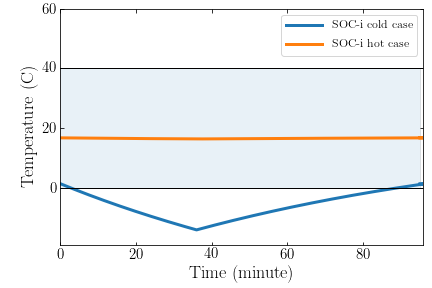
\includegraphics[width=0.45\textwidth, keepaspectratio]{figures/TempsPlot_SOCi-hotVScold.png} 
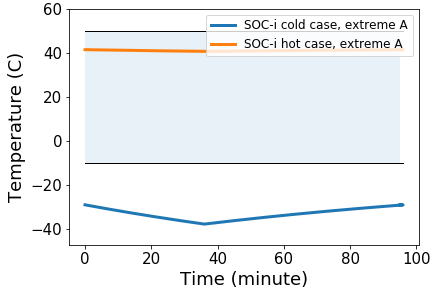
\includegraphics[width=0.45\textwidth, keepaspectratio]{figures/TempsPlot_SOCi-hotVScoldExtremeA.png} 

\caption{The impact of choosing extreme values of environmental conditions on SOC-i temperature,  
when assuming randomized satellite orientation (left), and with orientation that maximizes the temperature 
range between these so-called ``hot'' and ``cold'' cases (right). The temperature variation is compared to 
a typical battery operating temperature range (the blue horizontal band).  For hot case, there is no 
temperature variation with time because the assumed orbit has no eclipsed portion. 
\label{fig:SOCi1}}
\end{figure}


\section{Active temperature control \label{sec:active}} 

Given the allowed operating temperature ranges for satellite components (the most stringent requirement
comes from batteries, chosen here as 0--40 $^\circ$C for illustration), these results imply that 
low temperatures will be more worrisome than high temperatures. Motivated by this finding, we 
explored a model for active temperature control.




\subsection{A toy model for active temperature control } 

We developed a toy model for active temperature control that assumes an additional internal power 
dissipation whenever the satellite temperature drops below a pre-defined threshold. We investigated
cold case and three levels of power (2 W, 5, W, 10 W) that is applied whenever the temperature 
drops below 273 K (0 $^\circ$C). Results are shown in figure~\ref{fig:SOCi2}. 

Additional power can raise the satellite temperature by 5 to 11 degrees. The consumed power ranges
from 1.9 Wh to 4.3 Wh, and it is under the total available battery power (5.6 Wh for cold case and
$\eta_{cell}=0.2$; for hot, extreme case, it could be boosted to 18 Wh with $\eta_{cell}=0.3$). 
These results show that such an approach is a viable method for mitigating low temperatures.

\begin{figure}[t!]
\centering
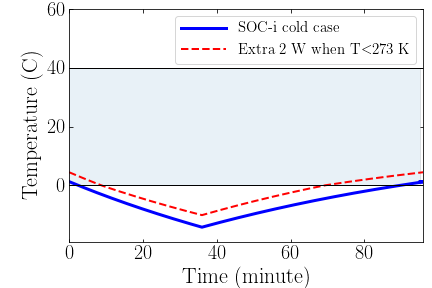
\includegraphics[width=0.3\textwidth, keepaspectratio]{figures/TempsPlotCompare_SOCi-cold-heated2.png} 
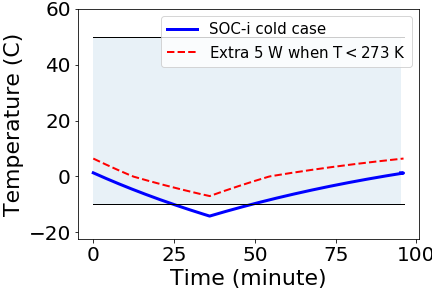
\includegraphics[width=0.3\textwidth, keepaspectratio]{figures/TempsPlotCompare_SOCi-cold-heated5.png} 
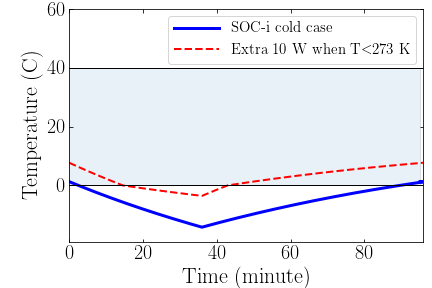
\includegraphics[width=0.3\textwidth, keepaspectratio]{figures/TempsPlotCompare_SOCi-cold-heated10.png} 
\caption{Illustration of the impact of active thermal control. A toy model assumes that whenever the satellite temperature
drops below zero $^\circ$C (273 K), an additional heating source with power of 2 W (left),  5 W (middle), or 10 W (right) contributes
to the heat balance. The blue lines correspond to the blue line in the left panel in figure~\ref{fig:SOCi1} (cold case) and the 
red dashed line is the corresponding temperature prediction with this additional heating power. The consumed power is about 
1.9 Wh, 3.4 Wh and 4.3 Wh, respectively (the total available battery power is 5.6 Wh). 
\label{fig:SOCi2}}
\end{figure}




\section{Conclusions \label{sec:conclusions}} 

We computed temperature variation with time for SOC-i satellite using a model with a single 
temperature that applies to the entire satellite surface at any given time, and a variety of input 
assumptions. 
 
We defined the so-called ``hot'' and ``cold'' cases and found that the low and high temperature 
extremes for a randomly oriented SOC-i satellite are $-$14 $^\circ$C and $+$17 $^\circ$C. When the 
satellite orientation is deliberately chosen to maximize the temperature extremes, the corresponding 
values are $-$38 $^\circ$C and $+$42 $^\circ$C. 

Within the model limitations, these estimates are accurate to within a few degrees. The results are 
sensitive to assumed specific heat, which we simply assumed to correspond to aluminum. 

Since it appeared that low temperatures will be more concerning than high temperatures,
we also explored a toy model for active temperature control that assumes an additional internal 
power dissipation whenever the satellite temperature drops below a pre-defined threshold. 
We found out that such an approach is a viable method for mitigating low temperatures.

Without more detailed and robust SOC-i orbit and orientation descriptions, this model cannot
be appreciably improved. Nevertheless, significant additional insight can be gained from Ansys
models that are capable of computing temperature field throughout the satellite body. For
external heat fluxes, values listed in Table~\ref{tab:inputflux} can be used but {\bf they need
to be corrected for different values of absorption coefficient ($\alpha$) for each surface 
material.} 

It would be prudent to first start with hot case because there is no temperature variation along
the orbit and thus much faster steady-state Ansys calculation can be utilized. Once that case is verified
to be in approximate agreement with the results presented here (in particular, we expect that
the mean external surface temperature of 17 $^\circ$C for random orientations should be reproduced
to within a few degrees), transient thermal analysis should be attempted for cold case. 


\vskip 0.2in 
\leftline{\bf References}
Gilmore, D. 2002, ``Spacecraft Thermal Control Handbook: Fundamental Technologies'', 2nd ed. Aerospace Press 

Hengeveld, D.W. et al. 2009, ``Hot- and Cold-Case Orbits for Robust Thermal Control'', Journal of Spacecraft and 
     \phantom{xxxxxx} Rockets,  Vol. 46, No. 6 

Jacques, L. 2009, ``Thermal Design of the Oufti-1 Nanosatellite'', Master Thesis, University of Liege

Kang, S-J. \& Oh, H-U. 2016, ``On-Orbit Thermal Design and Validation of 1 U Standardized CubeSat of STEP 
\phantom{xxxxxx}  Cube Lab'', 
        International Journal of Aerospace Engineering, Vol. 2016, Article 4213189

Kellens, A. 2018, ``Thermal design of the OUFTI-Next mission'', Master thesis, University of Liege
\end{document}



Orbit: permanently illuminated for hot case and max eclipse time for cold case. e
Internal power: full for hot, none for cold 


The mean albedo coefficient proposed by the European Cooperation for Space
Standardization (ECSS) is 0.3 but it is highly variable and depends on both the position on
Earth and time. For instance, a value of 0.05 corresponds to oceans while ice caps or high clouds
have an albedo coefficient of 0.6 [28].


More input parameters in Kang \& Oh (2016) paper. 


Lionel: hot and cold cases: deviations of at most 5 C from single-node analysis 

The parameters that are biased hot or cold are: 
1) Environmental Constants (Solar, Albedo, IR)    Table 
2)   Internal Power Dissipation
3)   Emissivity and Absorptivity for exposed surfaces:   alpha_S  alpha_IR   epsilon_T 
          add table with all kinds of materials 
4)   Spacecraft Orbital Orientation:   sun-asynchronous orbit, beta angle etc 

External surfaces emissivity/absorptivity values are not perfectly known and vary throughout the 
lifetime of the spacecraft (mainly an increase for a due to high reactive atomic oxygen present in 
the upper layers of the atmosphere) and are therefore subjected to the cold/hot case definition.



\section{The orbital $\beta$ angle}

The orbital $\beta$ angle is the angle between the solar vector and the orbital plane,  and varies from
$-90$ deg. to $+90$ deg. Satellites with positive $\beta$  appear to be going counterclockwise whereas negative 
$\beta$  indicate a clockwise direction, as viewed from the Sun. The satellite is exposed to more sunlight per orbit 
as $\beta$ angle increases, and eventually reaches constant sunlight exposure when $\beta = 90$ deg.
The input heat flux increases with $\beta$, that is, it's minimal for $\beta = 0$ deg.

$\beta$ is a function of both Sun's coordinates and orbital elements: 
\eq{
   \beta = \sin^{-1}\left[ \cos(\delta) \sin(i) \sin(\Omega-\Omega_{sun}) + \sin(\delta) \cos(i)  \right] 
} 

Here, $\Omega$ is the right ascension of the ascending node (RAAN).  Inclination $i=97$ deg for sun-synchronous
orbit at 550 km altitude. 
 
For the cold case, $\beta=0$. For the hot case and $h=550$ km, $\beta=67$ deg. 




\section{Hengeveld et al. (2009)} 

Hengeveld et al. 2009, ``Hot- and Cold-Case Orbits for Robust Thermal Control'',  
JOURNAL OF SPACECRAFT AND ROCKETS,  Vol. 46, No. 6


 
\end{document}

  

\section{Motivation} 

When designing a satellite, it is crucial to establish that the temperature variation for each component 
will be within its operating range. In practice, professional engineering tools and numerical analysis 
are used to analyze complex systems. Nevertheless, approximately correct temperature estimates 
and physical insight can be derived even using simple analytic models. 


\section{Simple thermal model for a spherical satellite} 

Consider a spherical satellite of radius $R$ and assume a uniform temperature over its surface
at any given time, $T(t)$. The temperature variation with time depends on the difference between
heat source, $Q_{in}$, and heat sink, $Q_{out}$, 
\eq{
\label{eq:dTdt}
              C  m {dT \over dt} =  Q_{in} - Q_{out}, 
}
where $C$ is the material heat capacity (e.g., for aluminium $C=921.1$ J kg$^{-1}$K$^{-1}$) and
$m$ is the satellite mass. The $Cm$ product is often called thermal inertia. Heat sources and sinks 
are measured in Watts (W = Js$^{-1}$). 

Assuming that the satellite is in vacuum, the heat sink is due to radiative loss, 
\eq{
\label{eq:Qout}
                 Q_{out} = A_s \epsilon_T \, \sigma T^4
}
where $A_s = 4\pi R^2$ is the satellite surface area, $\sigma=5.67\times10^{-8}$ Wm$^{-2}$K$^{-4}$ 
is the Stefan-Boltzmann constant,  and $\epsilon_T$ is the wavelength-averaged 
surface emissivity over the thermal flux distribution, and approximately equal to the emissivity
at the wavelength of the peak emission. From Wien's Law, this wavelength is equal to (3000 K$\mic$)/T
and thus for $T \approx 300$ K, $\epsilon_T$ is approximately equal to the material emissivity around 
10 $\mic$. Typical values of $\epsilon_T$  for materials used in satellite industry are in the range 0.8-0.9. 

The heat sources can include direct solar radiation, $Q_{sun}$, solar radiation reflected from Earth, $Q_{ref}$,
thermal infrared emission from Earth, $Q_{IR}$,  and internal power dissipation, $P_s$. When the satellite
is exposed to direct sunlight, the maximum possible heat source corresponds to 
\eq{
                   Q_{in}^{hot}  = Q_{sun} + Q_{ref} + Q_{IR} + P_s,
} 
while the minimum possible heating corresponds to 
\eq{
                   Q_{in}^{cold}  = Q_{IR}. 
} 

The two extremes, ``hot'' and ``cold'', should not be confused with ``hot'' and ``cold'' scenarios
that maximize/minimize the satellite temperature over an orbital cycle. 



\subsection{Heat sources} 

The time-averaged solar flux is about $F_{sun}$=1362 Wm$^{-2}$ and its spectral energy distribution peaks 
at wavelenghts of about 0.5 $\mic$ (yellow light; the Sun's surface temperature is about 5,800 K). Since 
the Earth's orbit is not circular, the solar flux varies from 1322 Wm$^{-2}$ in June to 1422 Wm$^{-2}$ in December, 
or by about 4\% around its mean value. The absorbed energy due to solar flux is then 
\eq{
                   Q_{sun}  = A_p \, \alpha_S  \, F_{sun}, 
} 
where  $A_p = \pi R^2$ is the satellite's projected surface area towards the Sun and $\alpha_S$ is the 
wavelength-averaged surface absorptivity over the solar flux distribution. As summarized by Kirchhoff's Law, 
$\alpha_S$ is approximately equal to the emissivity at 0.5 $\mic$, the wavelength of the peak of the solar 
spectral energy distribution. The low values of $\alpha_S$ imply high reflectivity and ``shiny'' surfaces. 

The fraction of solar flux reflected by Earth back towards the satellite is typically $\rho_E=0.3$, and it 
varies in the range $\rho_E=0.2-0.4$ across Earths' surface and oceans. The absorbed energy is then
\eq{
                    Q_{ref} =  A_p^{E}  \, \alpha_S  \, \rho_E  F_{sun} = \rho_E \, Q_{sun},
}
where it was assumed that Earth is so close to the satellite that it fills 2$\pi$ srad (``half the sky''). The 
correction for low-Earth orbit is smaller than the variation of $Q_{ref}$ due to variation of  $\rho_E$ across
Earth's surface\footnote{The so-called viewing factor is equal to $(R_E/R_E+h)^2 \sim 0.85$, where 
$R_E=6378$ km is the mean radius of the Earth and $h=550$ km is the assumed altitude of a low-Earth
orbit.}.  The projected surface area towards Earth, $A_p^{E}$, is equal to $A_p$ in case of spherical 
satellites.  

The thermal infrared flux emitted by Earth is about $F_{IR}$=239 Wm$^{-2}$, and it is equal to one quarter
(the ratio $A_p/A_s$ for Earth) of the absorbed solar radiation (about 70\% of $F_{sun}$=1362 Wm$^{-2}$ 
for $\rho_E=0.3$).  Given Earth's equilibrium temperature of $\approx$300 K, the spectral energy 
distribution of this radiation peaks at about 10 $\mic$. Therefore, 
\eq{
                    Q_{IR} =  A_p^{E} \, \alpha_{IR} \, F_{IR},
}
where $\alpha_{IR}$ is the wavelength-averaged surface absorptivity over the Earth's thermal flux distribution.
Given Kirchhoff's Law and the fact that the satellite and Earth's temperatures are similar, 
$\alpha_{IR} \approx \epsilon_T$. Due to varying properties of the Earth's surface (oceans, continents,
clouds), $F_{IR}$ can vary by about $\pm$10\% along the satellite's orbit. 

Note that all three heat sources are proportional to the projected area $A_p$ in case of spherical satellites.
When $\alpha_{IR} \approx \alpha_S$, $Q_{sun}$ is about twice as large as the sum of $Q_{ref}$ and $Q_{IR}$.  
For $R=0.095$ m, which gives $A_p$ equal to the largest projected area of a 2U CubeSat (=$2\sqrt{2}a^2$, 
where $a=0.1$m), and $\alpha_S = 0.9$, $Q_{sun}$ = 35 W.  

The internal power dissipation for a 2U CubeSat is of the order $P_s=10$ W. Therefore, $Q_{in}^{hot}$ = 62 W 
and $Q_{in}^{cold}$ = 6.1 W.    

\subsection{Internal power dissipation} 

Note a possible double counting of incoming energy, depending on how solar panels are treated.
If the solar panels are thermally decoupled from the satellite body, then $P_s=10$ W assumed above
is effectively an additional energy source. However, in 2U CubeSat case the solar panels are actually the 
satellite's sides and $P_s$ should be subtracted from $Q_{in}^{hot}$ (about 30\% of incoming flux is 
converted into electrical energy). Since energy must be conserved, the net effect is to spread the heating 
along the orbit and the total amount of absorbed energy per orbit remains same. Indeed, there is no 
reason to assume that $P_s$ must only contribute to $Q_{in}^{hot}$ -- it may as well contribute to 
$Q_{in}^{cold}$. 


\subsection{Equilibrium temperatures} 

The equilibrium temperature can be computed by assuming that the satellite is exposed to a constant 
heat source for an infinitely long time and thus $dT/dt=0$. It then follows from eqs.~\ref{eq:dTdt} and 
\ref{eq:Qout} that
\eq{
\label{eq:Teq}
                  T_{eq} = \left(  {Q_{in} \over A_s \, \epsilon_T \, \sigma} \right)^{1/4}. 
}
Note that the equilibrium temperature does not depend on satellite's thermal inertia (the product of 
mass and heat capacity). 

Assuming $Q_{in}^{hot}$ = 62 W and $Q_{in}^{cold}$ = 6.1 W, $T_{eq}^{hot} = 321$ K (48 C) and 
$T_{eq}^{cold} = 180$ K ($-$93 C) for $\epsilon_T=0.9$ and $R=0.095$ m ($A_s=0.02828$ m$^2$). 
This temperature range is much larger than the satellite temperature 
variation expected for oscillatory heating in a typical orbit, as discussed next. 


\subsection{Analytic solution for the temperature's return to its equilibrium value} 

Equation~\ref{eq:dTdt} can be recast using eqs.~\ref{eq:Qout}  and \ref{eq:Teq} as 
\eq{
\label{eq:dtaudx}
               {d\tau \over dx }  = 1 - \tau^4, 
}
where $\tau=T/T_{eq}$, $x=t/t_o$ and the time scale $t_o$ is given by 
\eq{
\label{eq:t0}
     t_o =   { C m \over A_s \, \epsilon_T \, \sigma \, T_{eq}^3}. 
}
The derivative $d\tau/ dx$ is positive when starting temperature $T_o=T(t=0)$ is
$T_o < T_{eq}$. Thus, when $Q_{in} = Q_{in}^{hot}$ and $T_{eq} = T_{eq}^{hot}$, the temperature
will be increasing with time, while for $Q_{in} = Q_{in}^{cold}$ and $T_{eq} = T_{eq}^{cold}$
the derivative is negative and the temperature decreases with time.

The simplified dimensionless differential equation \ref{eq:dtaudx} admits an implicit analytic solution:
\eq{
\label{eq:analytic}
{t \over t_o} = {1\over 2}\left[\arctan(\tau) - \arctan(\tau_o)\right] + {1\over 4}\left[\ln\left({\tau+1\over\tau_o+1}\right) - \ln\left({\tau-1\over\tau_o-1}\right) \right], 
}
where $\tau_o = T_o/T_{eq}$ is the initial condition. When $t \gg t_o$, $\tau$ asymptotically approaches unity. 
Figure~\ref{fig:analytic} illustrates solutions given by eq.~\ref{eq:analytic} for both $\tau_o<1$ and $\tau_o>1$. 
 
\begin{figure}[t]
\centering
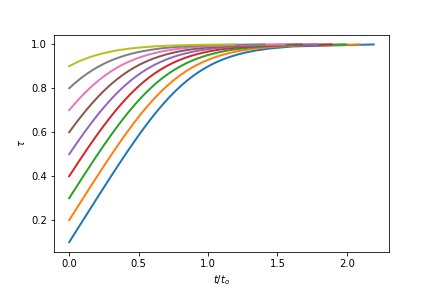
\includegraphics[width=0.45\textwidth, keepaspectratio]{analyticUp.png}
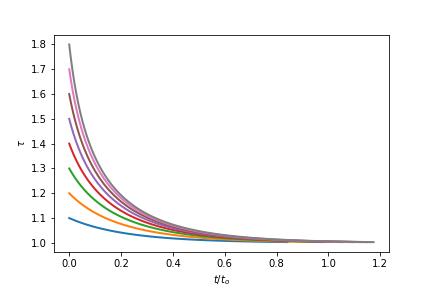
\includegraphics[width=0.45\textwidth, keepaspectratio]{analyticDown.png}
\caption{The analytic solution for dimensionless temperature parameter $\tau(t) = T(t)/T_{eq}$
as a function of  dimensionless time parameter $t/t_o$ for initial conditions with $\tau_o<1$
(left) and $\tau_o>1$ (right). Note that in both cases $\tau(t)$ asymptotically approaches unity,
that is, $T(t)$ asymptotically approaches $T_{eq}$. 
\label{fig:analytic}}
\end{figure}



\subsection{Temperature variation for a bistable heat source} 

Now consider a bistable heat source, such as a satellite in an orbit and a heat source periodically
switching between $Q_{in}^{hot}$ and $Q_{in}^{cold}$. Because corresponding equilibrium temperatures 
$T_{eq}^{hot}$ and $T_{eq}^{cold}$ are different, the implied time scales for temperature's return to its
equilibrium value, $t_o$ given by eq.~\ref{eq:t0}, will be different, too. Eq. ~\ref{eq:t0} implies that
the ratio of time scales in eclipse and when exposed to sunlight is 
\eq{
  { t_o^{cold} \over t_o^{hot} }= \left(Q_{in}^{hot} \over Q_{in}^{cold} \right)^{3/4} \approx 6. 
}
Therefore, the temperature gradient will be much higher when the temperature is rising. 

For a bistable heat source, the temperature at the end of the rising phase must be equal to the
temperature at the start of cooling phase and vice versa. As a result of this condition, the 
temperature will oscillate between two extremes, $T_{min}$ and $T_{max}$ with $T_{min} \ge T_{eq}^{cold}$ 
and $T_{max} \le T_{eq}^{hot}$.  Eq.~\ref{eq:analytic} appears too cumbersome to derive a closed-form
solutions for  $T_{min}$ and $T_{max}$; in practice,  $T_{min}$ and $T_{max}$ are determined iteratively. 

When thermal inertia is vanishing, the temperature will return to its equilibrium values essentially
instantaneously and most of the time the satellite temperature will be either $T_{eq}^{cold}$ or $T_{eq}^{hot}$. 
On the other hand, for infinitely large thermal inertia the temperature will assume an equilibrium
value that corresponds to the heat source averaged over orbit. For example, if the satellite spends
one third of the orbital period in eclipse, then
\eq{
\label{eq:TeqAve} 
      T_{eq}^{ave} = \left[ {1\over 3} \left(T_{eq}^{cold}\right)^4 +  {2\over 3} \left(T_{eq}^{hot}\right)^4 \right]^{1/4}. 
}
With $T_{eq}^{hot} = 321$ K and $T_{eq}^{cold} = 180$ K, $T_{eq}^{ave} = 293$ K (20 C). 

Realistic cases with thermal inertia between these two extremes are discussed next. 


\section{Discussion} 

\begin{figure}[t]
\centering
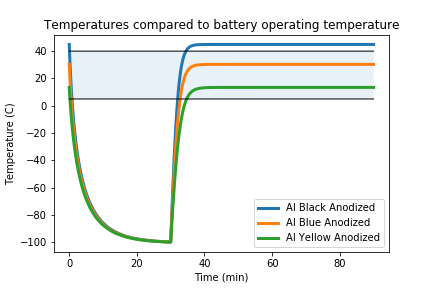
\includegraphics[width=0.31\textwidth, keepaspectratio]{Tt_C005.png}
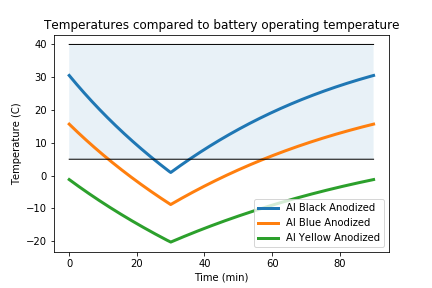
\includegraphics[width=0.31\textwidth, keepaspectratio]{Tt_SOCi.png}
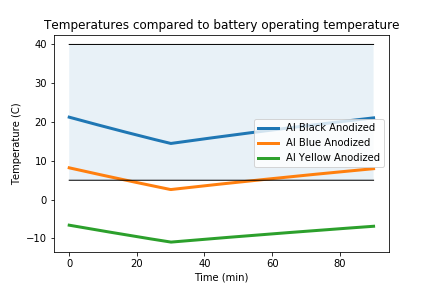
\includegraphics[width=0.31\textwidth, keepaspectratio]{Tt_C10.png}
\caption{The satellite orbital temperature variation as a function of the surface emissivity properties 
and thermal inertia. Three different types of anodized aluminum surfaces: black with $\alpha_S, \epsilon_T$ 
= (0.86, 0.86), blue: (0.67, 0.87)  and yellow: (0.47, 0.87).  The satellite is a hollow sphere with the radius 
of 0.095 m. The thermal inertia is controlled by the mass; left: low (0.05 kg), middle: medium (2.2 kg; 
the University of Washington SOC-i CubeSat satellite), right: high (10 kg; the solid aluminium sphere).
The temperature variation is compared to typical battery operating temperature range (the blue horizontal
band).  
\label{fig:Tt}}
\end{figure}


Figure~\ref{fig:Tt} shows the satellite orbital temperature variation as a function of the surface emissivity
properties and thermal inertia. The temperature variation is computed using analytic solution given by
eq.~\ref{eq:analytic} and emissivity properties corresponding to three different types of anodized aluminum 
surfaces (see figure caption). It is assumed that the orbital period is 90 min, with the eclipse lasting 30 min. 
The aluminium heat capacity is assumed and the thermal inertia is controlled by the satellite mass. 

For low thermal inertia (left panel), the temperature displays large variation, drops quickly to the cold 
equilibrium temperature and rises back even faster to the hot equilibrium temperature. For very high
thermal inertia (right panel) the temperature varies by only a few degrees around the value given by 
eq.~\ref{eq:TeqAve}. In the most realistic case shown in the middle panel, the temperature variation 
amplitude is about 20-30 degrees. 

This behavior is similar to potatoes taken from a hot oven: small satellites would cool faster 
than their scaled-up larger versions. However, here the difference in behavior is due to different 
thermal inertia for satellites that look identical from the outside (same size, shape and surface properties). 
Instead of small and large potatoes, a better analogy is solid and hollow potatoes of the same size.



 
\subsection{CubeSats are not spherical!} 



\begin{figure}[t]
\centering
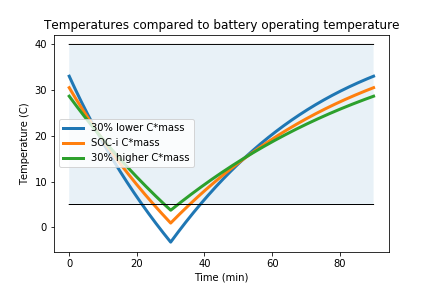
\includegraphics[width=0.45\textwidth, keepaspectratio]{Tt_SOCi_Cvariation30.png}
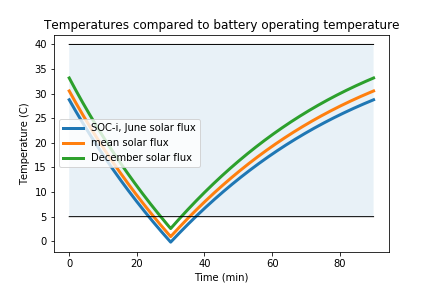
\includegraphics[width=0.45\textwidth, keepaspectratio]{Tt_SOCi_SolarFluxVariation.png}
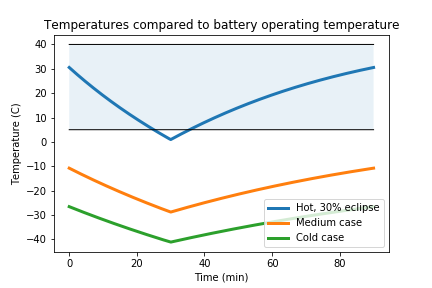
\includegraphics[width=0.45\textwidth, keepaspectratio]{Tt_SOCi_HotCold.png}
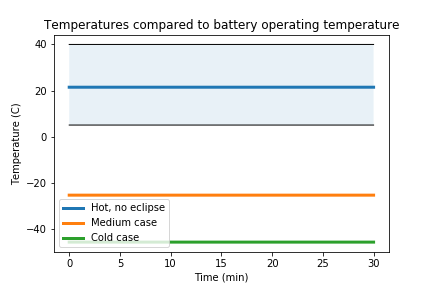
\includegraphics[width=0.45\textwidth, keepaspectratio]{Tt_SOCi_HotCold_noeclipse.png}
\caption{The impact of thermal inertia (top left), solar flux variation (top right) and effective projected area
(bottom left: 30\% of orbit in eclipse; bottom right: a polar orbit with no eclipse) on satellite orbital temperature 
variation (all for black anodized aluminum surface with $\alpha_S, \epsilon_T$  = 0.86, 0.86). In the bottom
panels, the effective projected area for the medium and cold case is assumed to be 2.0 times and 2.82 times 
smaller than for hot case, respectively (motivated by 2U CubeSat geometry). The temperature variation is 
compared to typical battery operating temperature range (the blue horizontal band).  
\label{fig:Tt2}}
\end{figure}


While CubeSat satellites are not spherical, if appropriate values of $A_s$, $A_p$ and $A_p^{IR}$ are used in 
computation, the observed temperature variation should be similar to that obtained with detailed numerical models. 
This simplified ``spherical cow'' model is suitable for studying the relative effects of surfaces with 
different emissivities, the effect of small changes in the solar flux between June and December\footnote{Everything
else being equal, the $\pm$4\% variation in the solar flux corresponds to about $\pm$1\% variation in the
satellite (absolute) temperature, or a tempeerature variation of about $\pm$3 C.} , the impact of thermal 
inertia, and as a ``sanity check'' for results obtained with detailed numerical models. Examples of 
such studies are shown in Figure~\ref{fig:Tt2}; the dominant effect for non-spherical satellites such as
2U CubeSat, is the impact of orientation on projected surface area. 

For a 2U CubeSat with the side length $a$ m, the smallest project area is $A_p^{min}$ = $a^2$ and
the largest projected area is $A_p^{max}$ = $2\sqrt{2}a^2$, a variation of about a factor of 3. With $A_s=10 a^2$,
the ratio $A_s/A_p$  varies between 3.5 and 10 (recall that $A_s/A_p=4$ for a sphere).  Therefore, if the 
largest possible projected area of a 2U CubeSat is oriented towards the Sun, the results will be similar to 
the spherical case with $a_{sphere} = 0.95 a$. In case of  the minimal projected area for intercepting incoming 
radiation, given that $T_{eq} \propto (A_p/A_s)^{1/4}$ (see eq.~\ref{eq:Teq}), the equilibrium temperature will be 
27\% lower than for the maximal projected area. Therefore, the CubeSat orientation with respect to 
the Sun and Earth can have a non-negligible effect on resulting temperature -- of the order 100 C. 
Note, however, that the variation of a 2U CubeSat temperature along the orbit due to varying satellite 
orientation will have a smaller amplitude due to finite thermal inertia and the heating contribution of 
internal power dissipation (if it doesn't depend on orientation), see the bottom panels in Figure~\ref{fig:Tt2}. 

It is also important to recognize that within a satellite some components could achieve temperatures 
higher than $T_{max}$ (components close to the locations of internal power dissipation) and lower than 
$T_{min}$  (components close to radiating walls in eclipse). To obtain temperature variation for 
individual components, an professional tool (e.g., Thermal Desktop, Ansys) and numerical computations 
need to be employed. Nevertheless, the essential impact of thermal inertia on the amplitude of temperature 
variation will remain. 


\vskip 0.2in 
%\newpage 
\leftline{Acknowledgments} 

The original version of the modeling code, based on a numerical solution of the 
differential equation \ref{eq:dTdt}, was contributed by Haley Stewart (University of Washington).
I thank the University of Washington SOC-i team, in particular Boone Tate, Henry Brown 
and Charlie Kelly, for access to technical parameters describing their 2U CubeSat named SOC-i. 
 
%\software{numpy \citep{numpy}, scipy \citep{scipy}, pandas \citep{pandas}, astropy \citep{astropy-1, astropy-2}, matplotlib \citep{matplotlib}, corner \citep{corner}, seaborn %\citep{seaborn}, astroML \citep{2012cidu.conf...47V}}

%\bibliographystyle{aasjournal}
%\bibliography{ref}{}
%\input{appendix}


 
\end{document}

  